\documentclass[a4paper]{article}
\usepackage{amssymb}
\usepackage{graphicx}
%\usepackage{hyperref}
\usepackage{microtype}
\usepackage{amsmath, amsthm, amssymb} 

\title{H09M0A P\&D Embedded Systems and Multimedia}
\author{Seppe Iven - r0370830 \\ Koen Goetschalckx - r0375967}
\begin{document} 
\maketitle
\begin{center} Yu-Hui Huang, Johan Van Rompay, Hugo Van hamme
\end{center}

\section{Introduction}
This is an intermediate report about the MATLAB implementation of the P\&D assignment on subband coding, about the implementation of a speech codec. The main techniques used to create the codec are subband filtering and adaptive quantization, with the goal of compressing a stereo audio signal. The MATLAB implementation uses fixed point numbers to mimic the working of a DSP. The parameters can be set in a flexible manner with the eye to optimal speech quality.\\

This report first mentions the required specifications followed by the explanation of QMF filterbanks and adaptive differential quantization. Next, it shows the general MATLAB structure of the implementation of the assignment and what all MATLAB scripts and functions do. It then handles the PESQ scores and the criterion for optimal values. After this, this report gives the current set of optimal values. The final part of this paper is about the PESQ score for audio that has been encoded and then decoded with this implementation and a general conclusion.

\section{Main design specifications}
The following list contains the specifications that the design of the codec has to meet.

\begin{itemize}
\item It accepts stereo signals
\item The sampling frequency is 8 kHz
\item The bit rate is 24 kbit/s per channel codec, with good to very good speech quality
\item The implementation consists of a QMF tree-structured filterbank with polyphase implementation
\item An adaptive differential quantization scheme should be used for every subband signal
\item The filterbank of the codec consists of a minimum of 4 subbands
\item The total delay of the coder and decoder must not exceed a certain threshold: the entire one way communication delay (ADC, coding, encryption, decryption, decoding, DAC) should be less than 150 ms. This puts a maximum on the number of subbands, on the complexity of the filters and on the buffer size in the cryptography section. Note that the encryption and decryption functionality is provided by another group and is not a part of this assignment.

\end{itemize}


\section{Splitting into subbands: QMF}
An input audio stream is split into subbands by using a Quadrature Mirror Filter bank.
A QMF filter bank consists of a low-pass and high-pass filter $H_0(z)$ and $H_1(z)$. These split the audio file into a low-frequency and a high-frequency part. Such filter bank is used to efficiently create a two-way filter bank. A recursive implementation is used to split an audio file into four subbands as shown by figure \ref{fig:qmfrecursive}.\\
\begin{figure}[hbt]
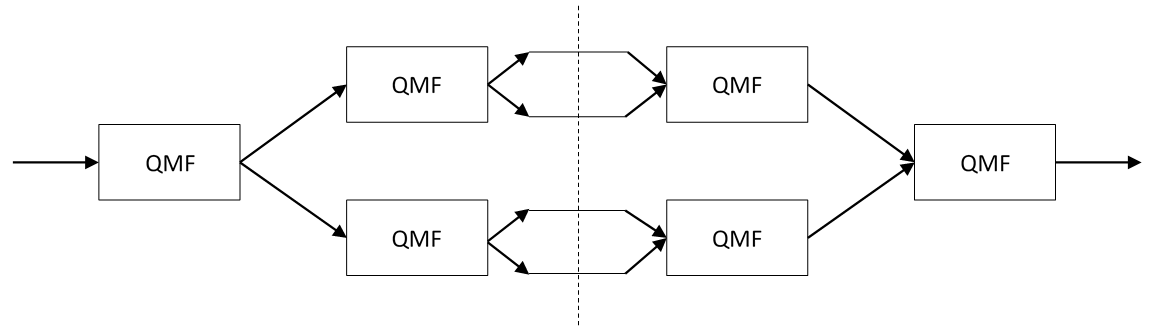
\includegraphics[width = \textwidth]{qmfrecursive}
\caption{four subbands QMF filter bank}
\label{fig:qmfrecursive}
\end{figure} \\
QMF filters have some special properties:
\begin{itemize}
\item if $H_0(z)$ is a QMF filter, then $H_1(z) = H_0(-z)$ has the frequency response of $H_0$ mirrored around $\pi/2$.
\item if $H_0(z)$ is a QMF filter, then analysis filters $H_0(z)$ and $H_1(z) = H_0(-z)$ and synthesis filters $F_0(z)=H_1(-z)=H_0(z)$ and $F_1(z)=-H_0(-z) = -H_1(z)$ form an alias-free filter bank.
\end{itemize}

The second property indicates that a complete alias-free QMF filter bank can be defined by $H_0(z)$ alone. For the filter to be linear phase, this $H_0$ should be chosen symmetrical. Also, the filter should have an even amount of taps to avoid distortion at half the Nyquist frequency. The first property indicates that if $H_0$ is a good low-pass filter, then $H_1$ is a good high-pass filter. \\

Given these properties and constraints, a simple polyphase implementation for a QMF filter bank can be designed, and is shown in figure \ref{fig:qmf}. The polyphase decomposition of $H_0(z)$ is:\\
\begin{center}
$H_0(z)$ = $E_0(z^2) + z^{-1} E_1(z^2)$ \\
\end{center}
From the first property, it follows that: \\
\begin{center}
$H_1(z)$ = $E_0(z^2) - z^{-1} E_1(z^2)$ \\
\end{center}
This leads to the efficient implementation of the filter bank shown in figure \ref{fig:qmf}.

\begin{figure}[hbt]
\includegraphics[width = \textwidth]{qmf}
\caption{Polyphase implementation of QMF filter bank}
\label{fig:qmf}
\end{figure}

For this project, both symmetric and asymmetric, where only one of the output bands of a QMF block are split further, structures were considered. Although for example 5 subbands created by always splitting the lower frequency band, may possibly have lead to better results, further use and study of these asymmetric structures were canceled as the teacher assistant said these were never considered previously and would lead to more complex C implementation. Thus, the final structure consists of QMF filter bank symmetrically splitting the signal into four subbands, as in figure \ref{fig:qmfrecursive}. Experiments show that four subbands can give good results in PESQ scores (discussed later). Eight or more subbands are thus not necessary but unwanted due to higher delay and computation complexity.

\section{Adaptive differential quantization}
After filtering into subbands, the data is now encoded with an adaptive differential quantization scheme. The quantizer can be seen in figure \ref{fig:quantization} and the dequantizer in figure \ref{fig:dequantization}. They contain the following signals:

\begin{itemize}
\item s(n) is the (serial) input signal
\item d(n) is the difference signal between the input signal and the prediction of the signal
\item z(n) is the quantized difference signal. This is also the output signal of the quantizer, hence the 'differential' in the name
\item d'(n) is the difference signal after quantization and dequantization. It thus resembles d(n) but is not exactly the same value
\item s'(n) is the sum of d'(n) and the prediction. It thus resembles s(n) but is not exactly the same value
\item s*(n) is the prediction of the next input signal 
\end{itemize}

The step size is adaptive and based on the last values of d'(n) and a parameter $\phi$. The amount of values that influence the step size, is determined by a parameter 'buffer\_length'. Step size is calculated as follows:
\begin{equation*}
stepsize = round\_to\_zero(\phi*mean(abs(D'(n))))
\end{equation*}
Herein D'(n) contains the last buffer\_length values of d'(n). The mean should be zero, thus this equals the first central moment. This is chosen instead of the variance for easy of calculation. \\
The reason of the use of d'(n) instead of d(n) is because the dequantizer only knows d'(n) and not d(n). For the same reason, the prediction is based on s'(n) and not in s(n). The prediction is a simple first order prediction, defined by the previous approximation of the signal s'(n) and a parameter $\mu$:
\begin{equation*}
s^*(n) = \mu*s'(n-1)
\end{equation*}
The dequantizer can reconstruct s'(n) based on the z(n) it receives. The system is thus lossy, since it cannot reconstruct the exact signal s(n). The benefit of this system is that the only transmitted signal is z(n), whose range is normally smaller than the range of s(n). Thus less bits are needed for encoding and transmitting z(n) than for s(n) and lossy compression is realized.
\begin{figure}[hbt]
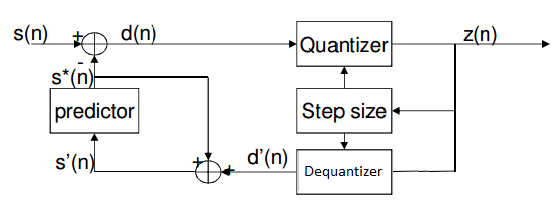
\includegraphics[width = \textwidth]{Quantization.png}
\caption{The Adaptive Differential Quantization scheme}
\label{fig:quantization}
\end{figure}
\begin{figure}[hbt]
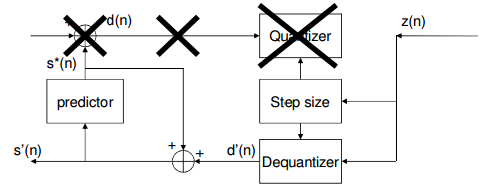
\includegraphics[width = \textwidth]{Dequantization.png}
\caption{The Adaptive Differential Dequantization scheme}
\label{fig:dequantization}
\end{figure}

Both the quantizer and dequantizer are initialized with the initial prediction $s^*(0) = 0$ and the initial $stepsize(0) = 1$.

\section{MATLAB structure - Implementation overview}
This section gives a brief explanation of the used MATLAB files and their functionality.

\subsection{generate\_some\_params.m}
This script can be run to generate parameters used to call run.m

\subsection{run.m}
This is the main function used to divide an audio file into subbands, encode and decode those subbands, and synthesize them again to create an audio signal that closely resembles the original signal. Accepted audio files are .wav-files that are stereo or pairwise mono. The input audio file that should be used, has to be named 'input.wav'.\\

The input is scaled to a 16-bit signed integer. The input is then split into subbands by calling analysis.m. These subbands are first encoded by calling encode.m. The result that is now obtained, is the signal that would be saved or transmitted in real use. Next, the function decodes the result by calling decode.m. Finally, calling synthesis.m recombines the subbands and the PESQ score for the reconstructed audio file is calculated. For this calculation, only one channel is considered, because in most of the test files the two channels are the same (effectively mono). Even when this is not the case, a noticeable increase of score in one channel should lead to a similar increase in the other for real life signals.

\subsection{analysis.m}
This MATLAB function splits the stereo (or pairwise mono) channels into separate channels, and splits them into subbands by calling get\_subbands.m.

\subsection{get\_subbands.m}
This function recursively splits an audio signal into its subbands. It does this by applying polyphase QMF filters, as explained earlier in this paper. These filters are generated with a function that was given as part of the assignment and characterized defined by its parameters.\\

Convolutions are used to apply the filters. Since this is a sum of products, the output values exceed the 16-bit range. The output must thus be downscaled again. This downscaling is done by division of a power of two, so it is easily implementable as a bit shift. The exponent of two can be chosen, as it is a parameter of this function. It should however be chosen with respect to the filter length: longer filters add more numbers, creating a larger result and thus the need for more downscaling. The choice of exponent gives rise to a trade-off between clipping and quantization noise. An exponent that is too small leads to the former, while a too large exponent leads to relatively larger quantization noise.

\subsection{encode.m}
This function uses the earlier mentioned adaptive differential quantization method to compress an input signal. A parameter determines the maximum output and thereby the amount of bits needed. Larger values are clipped. This should be avoided by changing the other parameters. For analysis purposes, the function keeps track of the number of times the clippings happened. Input parameters $\phi$ and $\mu$ must be scaled to signed 16-bit integers.

\subsection{decode.m}
This function is the inverse of encode.m: it takes the output of the adaptive differential quantisation function and constructs s'(n), which approximate the original input signal s(n). Parameters $\phi$ and $\mu$ and 'buffer\_length' should be the same as those used for encoding with encode.m.


\subsection{synthesis.m}
This function is the inverse of get\_subbands.m: its inputs are the separate subbands and it combines (synthesizes) them into one signal. The filters used for this are the same QMF filters used for analysis, as explained earlier in the text. As in analysis.m, scaling is done to refit the values into the 16-bit range.

\section{SNR \& PESQ score}
The perceptual metric PESQ is used to grade the quality of the codec. It was decided to use PESQ instead of SNR since it takes features of the human hearing into account (such as masking). This is why the optimal values are chosen on basis of PESQ scores, and SNR is mainly ignored.

\begin{table}[bth]
\begin{center}
\begin{tabular}{ l|ll }
  File name & PESQ score & Segmental SNR \\
  \hline
  belasting & 3.35 & 17.9\\
  bir & 3.66 & 19.2\\
  f116 & 3.04 & 14.3 \\
  f216 & 2.97 & 17.8\\
  m116 & 3.38 & 14.0\\
  m216 & 3.43 & 14.0\\
  words\_f & 3.46 & 19.1\\
  words\_m & 3.28 & 18.2\\
  combined\_8000\_short & 3.34 & 15.5 \\
  combined\_8000 & 3.54 & 18.4\\
  \hline
\end{tabular}
  \caption{PESQ and segmental SNR scores for different audio files}
\label{tab:pesqscores}
\end{center}
\end{table}

The parameters are optimized by maximizing the PESQ score for the audio file 'combined\_8000\_short.wav'. This is a combination of the audio files 'm116.wav', 'f116.wav' and 'f216.wav'. This is preferred to a single file, since it contains more variation as training data. All audio streams were delivered at 16kHz sampling rate, but the system is designed for 8kHz. Using Audacity, an anti-aliasing filter with 70dB attenuation for frequencies above 4kHz was applied to these audio files, before downsampling them to 8kHz. The values in table \ref{tab:pesqscores} are obtained using run.m with these downsampled versions.

\section{Set of optimal values of controllable parameters}
This section handles all of the parameters that define the implementation of the speech codec. Please note that although these values are currently our optimal values, they may be subject to changes in the future. This can be because of changes in the code, or because better values are found by (brute force) searching.\\

The QMF filters generated with the given function QMF\_design.m are characterized by the following parameters:

\begin{itemize}
\item The sampling frequency, which is mandatory 8 kHz
\item The total transition width of the prototype filter. This is default at a tenth of the sampling rate, and thus we have left it at 800
\item The minimum stopband attenuation of the prototype filter, which we have left at the default value of 60 dB for the first filter and changed to 50dB for the following filters
\item The frequency step for finding the optimal cut-off frequency, which we have left at the default value of 10
\item The maximum number of iterations, which we have at 600
\item The filter lengths, which we have at 64 for the filter at the first depth and 32 for the filters at the second depth. We have chosen these lengths as a compromise between filter quality and implementation delay
\
\end{itemize}

The encoding parameters $\mu$, $\phi$, buffer\_length and the number of bits per sample can be different for each subband. The values for all these parameters are listed in tables \ref{tab:parametervalues}. Table \ref{tab:scalingparameters} shows the amount of scaling used after the convolutions in each QMF filter.

\begin{table}[h]
\centering
\begin{tabular}{l|cccc} 
band frequency & lowest & low & high & highest \\ 
\hline 
\#bits & 5 & 4 & 3 & 0 \\ 
$\mu$ & 19660 & 1638 & 31129 & / \\  
$\phi$ & 8192 & 16384 & 29490 & / \\  
buffer\_length & 10 & 10 & 10 & / \\  
\hline 
\end{tabular}
\caption{Current optimal values of encoding parameters}
\label{tab:parametervalues}
\end{table}
\begin{table}[h]
\centering
\begin{tabular}{c|ccc}
scalings & lower frequencies & • &  higher frequencies \\ 
\hline 
depth 1 &  • & 17 & •  \\ 
depth 2 &  15 & • & 16  \\ 
\hline 
\end{tabular} 
\caption{Current scaling parameters (\#bits to shift)}
\label{tab:scalingparameters}
\end{table}
Lower subbands have more bits per sample, since they are more important to the human hearing. Notice that the highest frequencies are simply thrown away. Finding the other values started by chosing the values for the scaling, because these give very high differences in PESQ scores. One division by 2 (one bitshift) too many results in a lower amplitude of the signal, one too few leads to clipping and thus distortion. Next the buffer\_lengths were changed. The length for the lowest frequency made a large difference. The others did not have much influence and were thus set to the same value for easy implementation. From this point on $\mu$, $\phi$ and buffer\_length values were changed one by one, always selecting a value that increased the PESQ score on combined\_8000\_short.wav. This lead to mentioned values.

\section{Delay of the implementation}
The filters used in the QMF filter bank lead to a delay. For each depth in the filterbank, the delay is given by $delay_i = (n_i-1) / sample\_rate_i$ with $i$ the depth, $n_i$ the amount of filter taps at this depth and $sample\_rate_i$ the sample rate at this depth, which is equal to the original sample rate divided by $2^{i-1}$. With filters of 64 and 32 taps, the delay becomes:
\begin{equation*}
delay = \frac{(64-1)}{8000 Hz} + \frac{(32-1)}{4000 Hz} = 15.625 ms.
\end{equation*}

\section{Conclusion}
This intermediate paper was about the MATLAB implementation of the P\&D assignment on subband coding, about the implementation of a speech codec. The paper discussed the design specifications, splitting an audio signal into subbands with QMF and quantizing it with an adaptive differential quantization scheme. It then explained the MATLAB structure and scripts. The MATLAB functions work with fixed point values. This simulates the working on a DSP. All performance results should therefore not change when the system is run on a DSP. The achieved PESQ scores (2,73 to 3,54) were shown and indicate good performance. The optimal values of the parameters were found by searching for the highest PESQ score by changing the parameters. Finally, the delay of the implementation was briefly discussed and calculated to be less than $16ms$. This leaves $134ms$ for the encryption and decryption.
\clearpage
\section{References}
\begin{itemize}
\item S. K. Agrawal and O. P. Sahu, Two-Channel Quadrature Mirror Filter Bank: An Overview, 23/03/2016,
\texttt{http://www.hindawi.com/journals/ isrn/2013/815619/}
\item -, Audacity, 25/03/2016, \texttt{http://www.audacityteam.org/}
\end{itemize}
\end{document}